%!TEX root = ../report.tex

\section{Kraft}

\begin{wrapfigure}{r}{0.5\textwidth}
    \begin{center}
        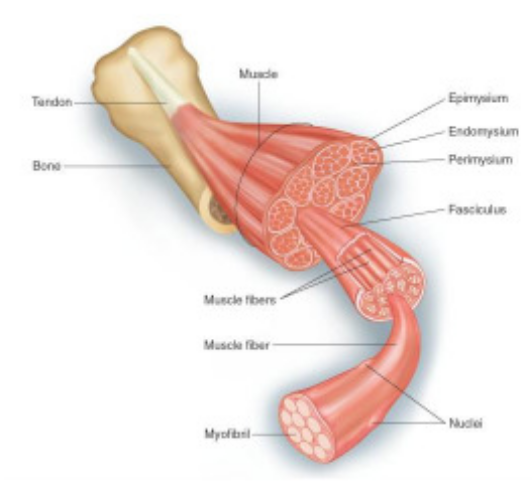
\includegraphics[width=0.48\textwidth]{pictures/muskeln}
    \end{center}
\end{wrapfigure}

Beispiele:
\begin{itemize}
    \item einmalig maximale Kraft (Gewichtheben)
    \item schnell und viel Kraft (Ringen, Hochsprung)
    \item Kraft aufrecht erhalten (Brücke)
\end{itemize}

Anatomische Grundlagen:
\begin{itemize}
    \item grundsätzlich drei Komponenten: Muskel, Sehne, Knochen
    \item Muskel bestehen aus:
    \begin{itemize}
        \item Muskelfaserbündel
        \item Muskelfaser
        \item Myofibrille
        \item Sarkomer
        \item Aktin-Myosin
    \end{itemize}
\end{itemize}

\begin{figure}[h]
\begin{tabular}{|c|c|c|c|}
 \hline
Kontraktionsform & Arbeitsweise & Ansatz / Ursprung & Beispiel Liegestütze \\ \hline \hline
konzentrisch & überwindend & Wird kleiner & Von Boden in Stütz \\ \hline
exzentrisch & nachgebend & Wird größer & Von Stütz auf Boden \\ \hline
isometrisch & haltend & Bleibt gleich & Halten des Stützes \\ \hline
\end{tabular}
\caption{Aktionsformen der Muskeln}
\end{figure}

\subsection{Struktur der Kraft}

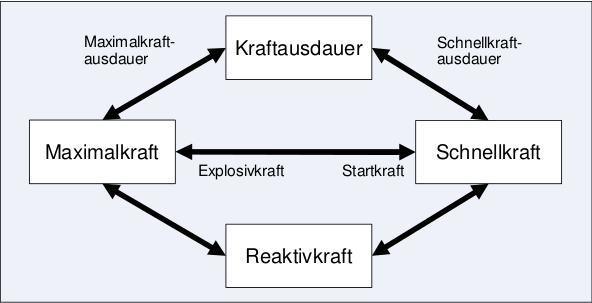
\includegraphics[width=0.9\textwidth]{pictures/kraftstruktur}

\subsection{Determinanten der Kraft}
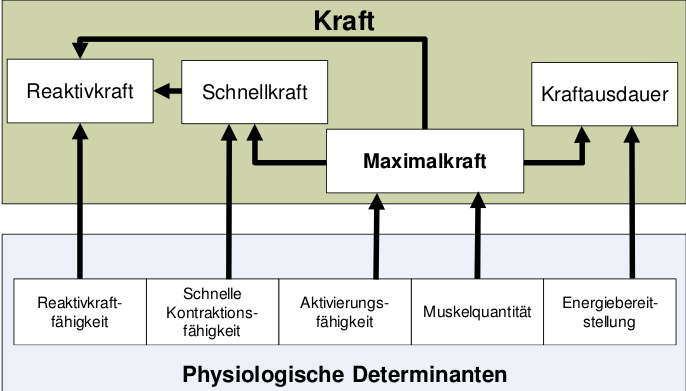
\includegraphics[width=0.9\textwidth]{pictures/kraft_determinanten}

\subsection{Maximalkraft}

[placeholder] % otherwise figure is not at correct position

\begin{wrapfigure}{r}{0.5\textwidth}
    \begin{center}
        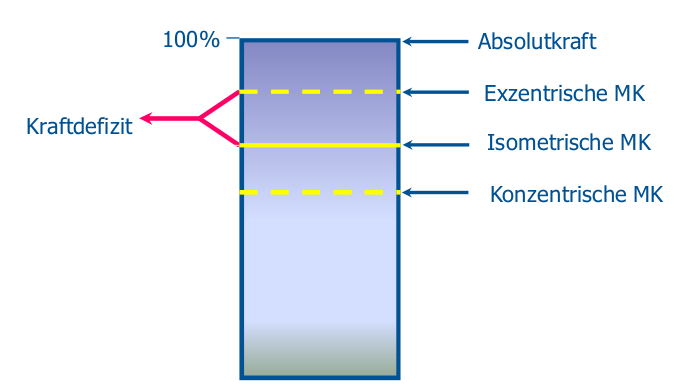
\includegraphics[width=0.48\textwidth]{pictures/maximalkraftvarianten}
    \end{center}
\end{wrapfigure}

[placeholder] % otherwise figure is not at correct position

\begin{itemize}
    \item Definition: Maximalkraft ist die höchstmögliche Kraft, die vom Nerv-Muskel-System willentlich gegen einen Widerstand erzeugt werden kann
    \item 1er-Maximum (1RM = 1 Repetition Maximum) = konzentrische Maximalkraft über volle Bewegungsamplitude
    \item Relativkraft = 1RM / Körpergewicht
    \item bestehend aus:
    \begin{itemize}
        \item Muskelquerschnitt \& Faserzusammensetzung
        \item Willkürliche Aktivierungsfähigkeit
    \end{itemize}
    \item Absolutkraft: Nur durch maximale elektrische Stimulation erreichbare Kraft. Willentlich nicht abrufbar.
    \item Kraftdefizit: $\frac{\text{Exzentrische MK} - \text{Isometrische MK}}{\text{Exzentrische MK}} \cdot 100 \%$
    \item in Praxis: Differenz zwischen isometrischer und exzentrischer MK
    \item Training:
    \begin{itemize}
        \item großes Kraftdefizit: willkürliche Aktivierungsfähigkeit verbessern
        \item kleines Kraftdefizit: Muskelquantität
    \end{itemize}
\end{itemize}

\subsection{Schnellkraft}

[placeholder] % otherwise figure is not at correct position
\begin{wrapfigure}{r}{0.5\textwidth}
  \begin{center}
    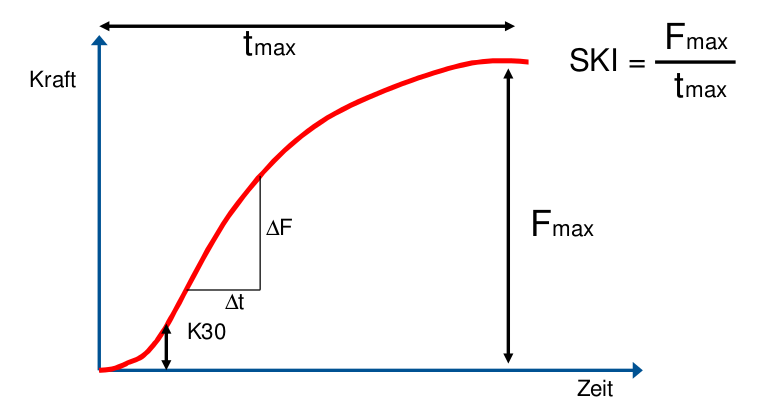
\includegraphics[width=0.48\textwidth]{pictures/kraftanstiegskurve}
  \end{center}
\end{wrapfigure}

\begin{itemize}
    \item Definition: Schnellkraft ist die Fähigkeit, einen möglichst großen Kraftstoß innerhalb einer zur Verfügung stehenden (kurzen) Zeit zu realisieren
    \item Teilaspekte:
    \begin{itemize}
        \item Startkraft (Fähigkeit sehr schnell Kraft zu entfalten, bsp: Boxen?)
        \item Explosivkraft (Fähigkeit großen/schnellen Kraftanstieg zu realisieren, bsp: Würfe, Stöße, Schüsse?)
        \item Dynamisches Kraftmaximum (Fähigkeit MK schnell zu realisieren, bsp: Ringen?)
    \end{itemize}
    \item Struktur der Schnellkraft: Maximalkraft + Schnelle Kontraktionsfähigkeit
    \item Schnelle Kontraktionsfähigkeit hängt ab von Muskelfaserzusammensetzung, Intermuskulärer und Intramuskulärer Koordination
\end{itemize}

\paragraph{Muskelfaserzusammensetzung}
\begin{itemize}
    \item Zusammensetzung genetisch determiniert
    \item Umwandlung praktisch nur Fast Twitch to Slow Twitch durch Ausdauertraining und Querschnittstraining
\end{itemize}
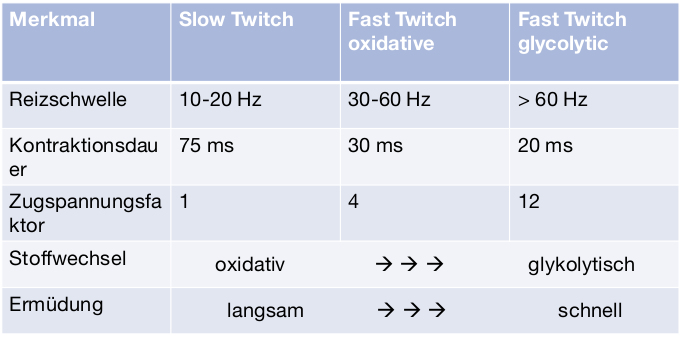
\includegraphics[width=0.9\textwidth]{pictures/muskelfaserzusammensetzung}

\paragraph{Intermuskuläre Koordination}
\begin{itemize}
    \item Zusammenspiel mehrerer Muskeln (Muskelabschnitte)
    \item fertigkeitsspezifisch
    \item kann als Synonym für ``Gute Technik'' betrachtet werden
    \item Grund warum Krafttraining nicht nur auf Stärkung der einzelnen Muskeln ausgelegt sein darf
    \item Beispiele: Fuß-, Knie- und Hüftstrecker bei Strecksprung
\end{itemize}

\paragraph{Intramuskuläre Koordination}
\begin{enumerate}
    \item Sequenzierung: Optimale Reihenfolge der Innervation der Muskelfasern
    \item Frequenzierung: Fähigkeit, den Muskel hochfrequent und nachhaltig zu innervieren
    \begin{itemize}
        \item Je nach Stärke der Erregung über die spinalen Synapsen, feuert ein Motoneuron mit unterschiedlicher Frequenz
        \item  Ab 55 Hz wird Maximale Kraftabgabe möglich
        \item  Bis zu 155 Hz sind möglich und erlauben schnellen Kraftanstieg
    \end{itemize}
    \item Rekrutierung: Fähigkeit, möglichst viele motorische Einheiten zur Kontraktion heranziehen zu können
\end{enumerate}
